\section{Umsetzung in TwinCAT} \label{Objektumsetzung in TwinCAT}
	\subsection{Allgemeine Struktur} \label{Objekt_Allgemeine Struktur}
		Die Programmierung der Objekte soll, ähnlich wie bei den Skills, möglichst einfach und übersichtlich gestaltet sein. Die Grundstruktur ist dabei identisch zu der der Skills. Ein Interface legt fest, welche Methoden und Eigenschaften ein Objekt zwingend besitzen muss.
		\\
		Die gemeinsamen Steuerungselemente und Betriebsvariablen werden durch Vererbung implementiert, sodass sie für alle Objekte einheitlich verfügbar sind (\ref{fig:Umsetzungsstruktur}). Unterschiede ergeben sich zwischen Aktoren und Sensoren: Während ein Aktor in der Regel umfangreicher definiert werden muss, kann ein Sensor deutlich einfacher und schlanker gestaltet werden.
		\\
		\begin{figure}[h!]
			\centering
			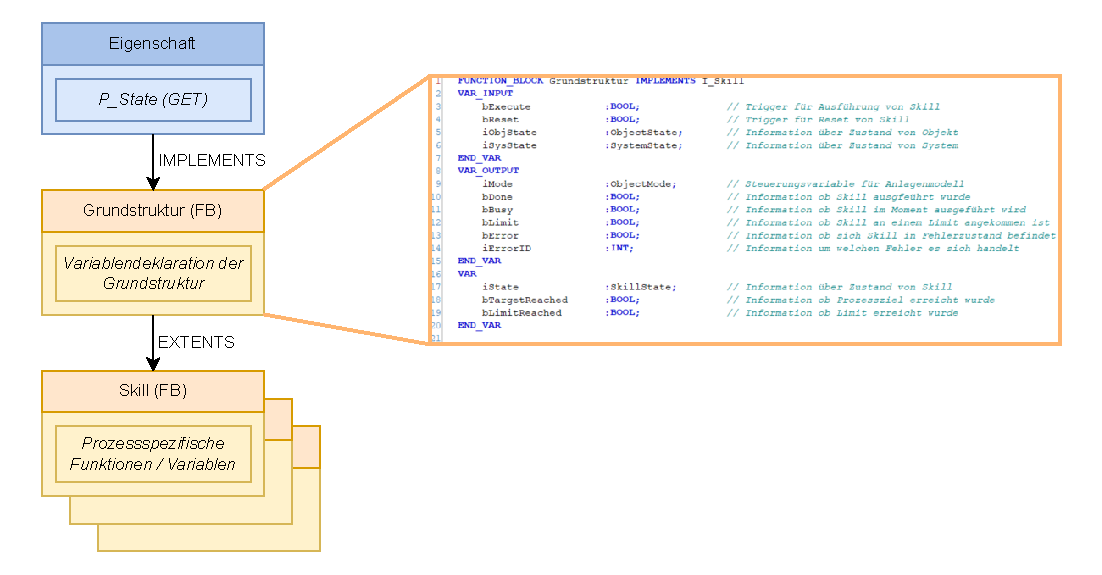
\includegraphics[width=0.8\textwidth]{07_Anlagenmodell/Umsetzungsstruktur}
			\captionsetup{justification=centering}
			\caption{Umsetzungsstruktur eines Objektes}
			\label{fig:Umsetzungsstruktur}
		\end{figure}
		
		\newpage
		
		Im Basis-Funktionsbaustein «\verb|FB_Basis_Objekt_Aktor|» (\ref{fig:FB_Basis_Objekt}) wurden die Betriebs-, Management- und Zustandsvariablen festgelegt. Auch hier zeigt sich die Parallele zum Aufbau des Skill-Basis-Funktionsbausteins, wodurch eine einheitliche Struktur gewährleistet wird.
		
		\begin{figure}[h!]
			\centering
			\fbox{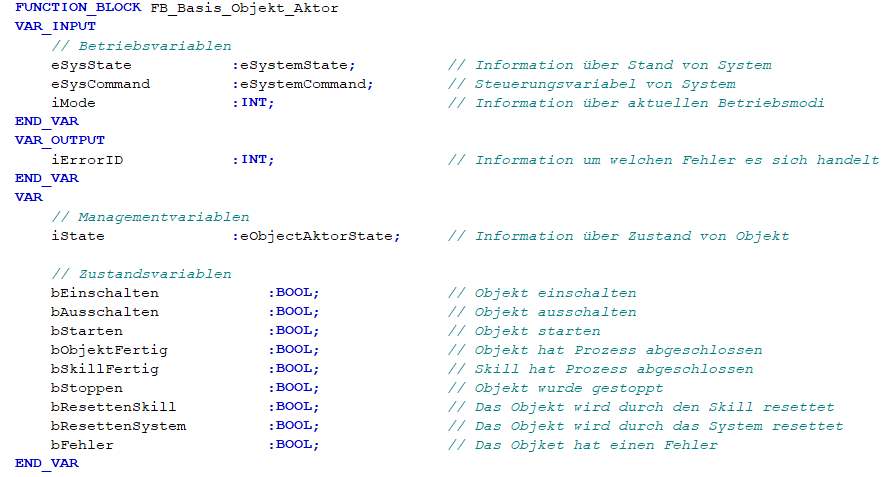
\includegraphics[width=0.8\textwidth]{07_Anlagenmodell/FB_Basis_Objekt_Aktor}}
			\captionsetup{justification=centering}
			\caption{Definitionen für Objekt-Basis-FB (Aktor)}
			\label{fig:FB_Basis_Objekt}
		\end{figure}
		
		Der Basis-Funktionsbaustein «\verb|FB_Basis_Objekt_Sensor|» verwendet dieselben Variablen wie der Aktor-Baustein. Allerdings wird für die Variable \verb|iState| der benutzerdefinierte Datentyp «\verb|eObjectSensorState|» verwendet. 
		\\
		Da ein Sensor im Vergleich zu einem Aktor weniger Zustände implementiert, sind bei den Zustandsvariablen deutlich weniger Transitionen abzubilden.
		\\
		Der Basis-Funktionsbaustein des Aktor-Objekt implementiert auch die Steuerungsmethoden der Objekte. Die Methoden wurden wie folgt umgesetzt:
		
		\begin{figure}[h!]
			\centering
			\begin{subfigure}[b]{0.4\textwidth}
				\centering
				\fbox{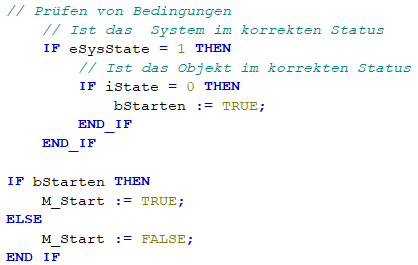
\includegraphics[width=\textwidth]{07_Anlagenmodell/MStart}}
				\caption{Methode: Start}
				\label{fig:Objekt_MStart}
			\end{subfigure}
			\hfill
			\begin{subfigure}[b]{0.3\textwidth}
				\centering
				\fbox{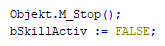
\includegraphics[width=\textwidth]{07_Anlagenmodell/MStop}}
				\caption{Methode: Stop}
				\label{fig:Objekt_MStop}
			\end{subfigure}
			\hfill
			\begin{subfigure}[b]{0.2\textwidth}
				\centering
				\fbox{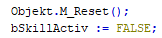
\includegraphics[width=\textwidth]{07_Anlagenmodell/MReset}}
				\caption{Methode: Reset}
				\label{fig:Objekt_MReset}
			\end{subfigure}
			\caption{Steuerungsmethoden eines Objektes}
			\label{fig:Steuerungsmethoden_Objekt}
		\end{figure} 
		
		Die Methode \verb|M_Start| (\ref{fig:Objekt_MStart}) überprüft zunächst den Status des Systems und anschliessend den Status des Objekts. Beide müssen sich im BEREIT-Zustand befinden, damit die Start-Variable aktiviert werden kann. Die Aktivierung der Variablen erfolgt nur, wenn sowohl das System als auch das Objekt die erforderlichen Voraussetzungen erfüllen.
		\\
		Die Stop-Methode (\ref{fig:Objekt_MStop}) kann ausschliesslich im LAUFEND-Zustand des Objekts ausgeführt werden. Für die Reset-Methode (\ref{fig:Objekt_MReset}) gibt es hingegen keine Bedingungen; sie kann unabhängig vom aktuellen Zustand des Systems oder des Objekts verwendet werden.
		
		\newpage
		
	\subsection{Aufbau des Grund-Objektes} \label{Grundobjekt_Aufbau}
		Das Grundobjekt definiert den Aufbau des Objektes, nachdem sich alle Objekte richten. Der Aufbau gliedert sich in fünf Hauptbereiche: Instanziierungen, Input-Command-Verwaltung, Interner Methodenaufruf, Datenerfassung und Zustandsmanagement.  
		
		\textbf{Instanziierungen:}
		\vspace{2mm} 
		\\
		Der Bereich wird genutzt, um notwendige, im Objekt-Funktionsbaustein instanziierte, TwinCAT-Funktionsbausteine aufzurufen. Diese werden nicht in Methoden aufgerufen, da es dabei zu Problemen kommen kann. Während der Entwicklung wurde die Erfahrung gemacht, dass beim Anwenden von Kommunikationsbausteinen für TCP/IP-Schnittstellen innerhalb einer Methode, Fehler auftreten können. Die Kommunikation ist nicht robust und es kann zu Fehlern kommen. Wenn der Kommunikationsbaustein aber im Objektbaustein selbst aufgerufen wird und die Methode nur auf das Eingangssignal einwirkt, ist die Funktionalität stabiler und reproduzierbarer. Bei der detaillierten Beschreibung der umgesetzten Objekte wird gezeigt, wie Funktionsbausteine aufgerufen werden. 
		
		\textbf{Input-Command-Verwaltung:}
		\vspace{2mm} 
		\\
		Die Input-Command-Verwaltung analysiert über die Variabel «\verb|eSysCommand|», ob das System einen Befehl vorgibt. Das System kann das Objekt einschalten, ausschalten, stoppen und resetten. Gewisse Befehle können nur ausgeführt werden, wenn sich das Objekt in einem bestimmen Zustand befindet.
		
		\textbf{Interner Methodenaufruf:}
		\vspace{2mm} 
		\\
		Wie der Name beschreibt, werden Methoden aufgerufen, welche nicht von aussen ausgeführt werden. Dabei kann es sich um Methoden handeln, welche zum Beispiel ausgeführt werden müssen, dass das Objekt eingeschalten wird und von «\verb|AUS|» zu «\verb|BEREIT|» wechseln kann.
		
		\textbf{Datenerfassung:}
		\vspace{2mm} 
		\\
		Der Bereich Datenerfassung wird der Prozess durchgeführt, welcher für die Erfassung von notwenigen Daten notwendig ist. Dazu gehört der Aufbau der Verbindung, das Auslesen von Daten und das Verarbeiten der Daten, so dass das Objekt damit arbeiten kann. Dies ist erforderlich, da manche Objekte bestimmte Informationen für Funktionen benötigen. Damit zum Beispiel ein Roboter-Objekt beurteilen kann, ob die Bewegung abgeschlossen wurde und dadurch in den Zustand «\verb|ABGESCHLOSSEN_INTERN|» wechseln kann, muss die aktuelle Position mit der gewünschten Position verglichen werden. Die aktuelle Position wird hierbei unter Datenerfassung erfasst. Es geht grundsätzlich um Daten, die während dem Betrieb des Objektes ausgewertet werden müssen. 
		
		\newpage
		
		\textbf{Zustandsmanagement: }
		\vspace{2mm} 
		\\
		Wie bei den Skills werden unter Zustandsmanagement die Zustände des Objektes umgesetzt. Für die Umsetzung wurde auch hier mit einer CASE-Anwendung gearbeitet.
		
		\begin{tabularx}{\textwidth}{@{}>{}p{16em} X@{}}
			Zustand 0 - \verb|AUS:| & 
			Der Zustand prüft nur, ob das Objekt durch das System eingeschaltet wird. Sobald die entsprechende Variabel aktiviert ist, wechselt das Objekt in den Zustand «\verb|BEREIT|» 
			\\
			Zustand 1 - \verb|BEREIT:| & 
			Das Objekt kann entweder gestartet, wieder ausgeschaltet oder in den Manuell-Modus geschalten werden. Beim Start des Prozesses durch einen Skill, wird die entsprechende interne Methode ausgeführt und der Zustand wechselt zu «\verb|LAUFEND|». Das Ausschalten kann nur durch das System gemacht werden.
			\\
			Zustand 2 - \verb|MANUELL:| & 
			Der Zustand implementier alle Funktionalität, welche das Objekt hat, so, dass diese manuell verwendet werden können. Dies kann zum Beispiel das manuelle Anfahren von Punkten mit dem Roboter sein.  
			\\
			Zustand 3 - \verb|LAUFEND:| & 
			Ein Objekt kann auf 2 Arten gestoppt werden, durch externen Einfluss oder das Objekt beendet den Prozess von selbst. Beides muss im Zustand überwacht werden. Beim Stoppen durch den Skill, wechselt das Objekt in den Zustand «\verb|ABGESCHLOSSEN_EXTERN|». Falls das Objekt selbst den Prozess stoppt, wechselt dieses in den Zustand «\verb|ABGESCHLOSSEN_INTERN|». Auch das System kann das Objekt stoppen, in diesem Fall wechselt das Objekt in den Zustand «\verb|GESTOPPT|», da dies ein Stoppen ausserhalb des ordentlichen Prozesses darstellt. Wie der Stop-Prozess innerhalb des Zustandes umgesetzt wird, kann von Objekt zu Objekt unterschiedlich sein.
			\\
			Zustand 4 - \verb|ABGESCHLOSSEN_INTERN:| & 
			Im Zustand wird auf den Reset-Befehl des Skills gewartet. Sobald dieser erkannt wird, wechselt das Objekt auf «\verb|BEREIT|». 
			\\
			Zustand 5 - \verb|ABGESCHLOSSEN_EXTERN:| & 
			Im Zustand wird auf den Reset-Befehl des Skills gewartet. Sobald dieser erkannt wird, wechselt das Objekt auf «\verb|BEREIT|».
			\\
			Zustand 6 - \verb|GESTOPPT:| & 
			Im Zustand wird auf den Reset-Befehl des Skills gewartet. Sobald dieser erkannt wird, wechselt das Objekt auf «\verb|BEREIT|».
			\\
			Zustand 7 - \verb|FEHLER:| & 
			Im Zustand wird auf den Reset-Befehl des Skills gewartet. Sobald dieser erkannt wird, wechselt das Objekt auf «\verb|BEREIT|».
			\\
		\end{tabularx}
		
		\newpage
		
	\subsection{Erarbeitete Objekte} \label{Objekt_Erarbeitet}
	
		\textbf{Objektklasse für UR5:} \verb|FB_Roboter|
		\vspace{2mm}
		\vspace{-10mm}  
		\\
		\begin{wrapfigure}{r}{0.5\textwidth}
			\centering
			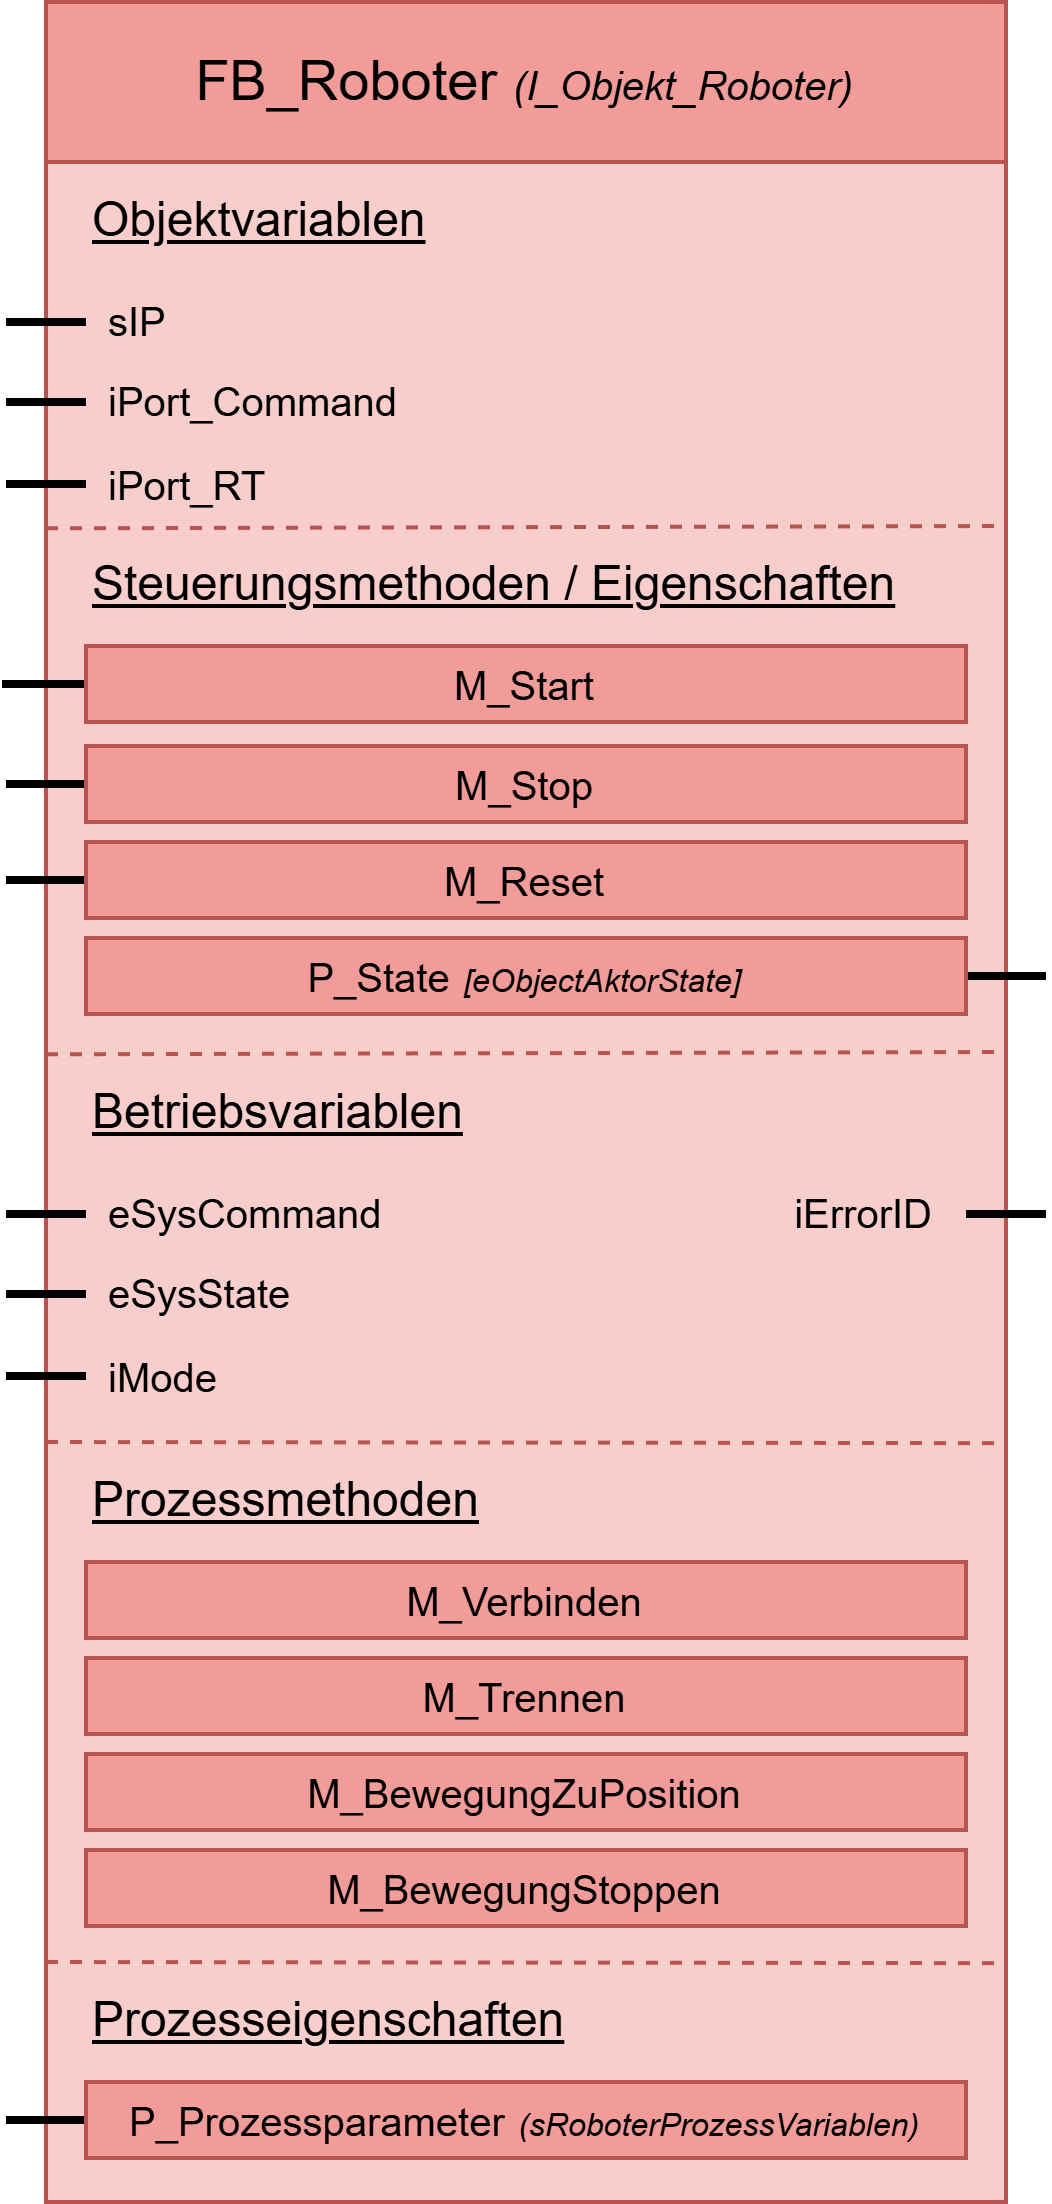
\includegraphics[width=0.45\textwidth]{07_Anlagenmodell/FB_Roboter}
			\captionsetup{justification=centering}
			\caption{Umsetzungsstruktur von Roboter-Objekt}
			\label{fig:Umsetzungsstruktur_Roboterobjekt}
		\end{wrapfigure} \par
		Die Objektklasse (\ref{fig:Umsetzungsstruktur_Roboterobjekt}) implementiert das Interface «\verb|I_Objekt_Roboter|», welches die Steuerungselemente des Objektklasse vorgibt. Als Objekt-Eingangsvariablen benötigt die Objektklasse eine IP-Adresse und zwei Port-Angaben. Die genaue Definition dieser Angaben wird in den folgenden Seiten erklärt. Es gibt keine Objekt-Ausgangs-variablen, welche mit EA-Klemmen verbunden werden müssten. Die Verbindung zum Roboter wird über TwinCAT-Funktions-bausteine durchgeführt, welche gleichzeitig auch die direkte Schnittstelle darstellen.
		\\
		Die Steuerungs- und Betriebsvariablen bleiben unverändert zum Basis-Funktions-baustein. 
		\\
		Als Prozessmethoden wurden \verb|M_Verbinden|, \verb|M_Trennen|, \verb|M_BewegungZuPosition| und \verb|M_BewegungStoppen| definiert. Diese Methoden decken die Grundfunktionen der Schnittstelle zum Roboter und dessen Funktionalität ab, um die definierte Anwendung umsetzen zu können. Damit weitere Funktionalitäten abgebildet werden könnten, müssten weitere Methoden hinzugefügt werden. Die Prozesseigenschaften bestehen aus den Prozessparametern, die für eine Punkt-zu-Punkt-Bewegung des Roboters benötigt werden.
		\\
		\\
		\\
		Wie bereits in Kapitel \ref{Anlagenkomponenten} angesprochen, besitzt der UR5 eine TCP/IP-Schnittstelle. Unterschiedliche Ports haben dabei unterschiedliche Funktionen (\ref{fig:Verbindungsports}). 
		
		\begin{figure}[h!]
			\centering
			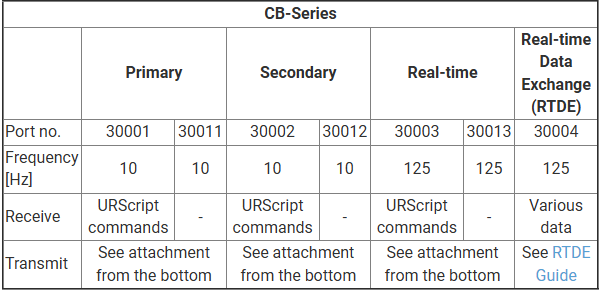
\includegraphics[width=0.75\textwidth]{07_Anlagenmodell/UR5_Ports}
			\captionsetup{justification=centering}
			\caption{UR5-Verbindungsports}
			\label{fig:Verbindungsports}
		\end{figure}
		
		\newpage
		
		\begin{bfhNoteBox}
			Beim eingesetzten Controller handelt es sich um einen CB2. Diverse Funktionalitäten der Schnittstellen oder zur Verfügung gestellte Dokumentationen richten sich an Controller ab Version CB3. Dies hat während der Entwicklung zu grossen Problemen geführt und viel Zeit in Anspruch genommen, vor allem bezüglich des Real-Time-Interfaces. Dieses wird in dieser Form nicht mehr unterstützt und wurde durch RTDE (Real-time Data Exchange) ersetzt, welche deutlich umfangreichere Funktionen bietet. Mittels Referenzprogrammen und alten Dokumentation konnte aber auch mit dem Real-Time-Interface gearbeitet werden.
		\end{bfhNoteBox}
		
		Über die Secundary-Schnittstelle (Port 30002) kann dem Roboter Befehle in der UR-eigenen UR-Script-Programmiersprache übergeben werden. Alle möglichen Befehle lassen sich aus der entsprechenden Dokumentation herauslesen (Anhang). 
		\\
		Über die Real-Time-Schnittstelle (Port 30003) kann ich Informationen über den Roboter in Echtzeit erhalten. Dabei erhält man ein Datenpaket von 812 Byte, bei welchem jede Position für eine bestimmte Information steht (\ref{tab:UR_Datenpaket}).
		
		\newcolumntype{L}[1]{>{\raggedright\let\newline\\\arraybackslash\hspace{0pt}}m{#1}}
		\begin{table}[ht]
			\scriptsize
			\centering
			\colorlet{BFH-table}{BFH-MediumBlue!10}
			\colorlet{BFH-tablehead}{BFH-MediumBlue!50}
			\begin{bfhTabular}{| l | c | c | c | L{6cm} |}
				Bezeichnung: 		& UR-Dt:	& TwinCAT-Dt:			& Byte:			& Beschreibung:
				\\\hline
				\verb|messageSize|	& INT			& LREAL				& 4 			& Gesamtlänger der Nachricht in Bytes
				\\\hline
				\verb|timestamp|	& DOUBLE		& LREAL				& 8 			& Zeitdauer seit Controller gestartet wurde
				\\\hline
				\verb|qTarget|		& DOUBLE		& LREAL				& 48 			& Zielposition der Gelenke
				\\\hline
				\verb|qdTarget|		& DOUBLE		& LREAL				& 48 			& Zielgeschwindigkeit der Gelenke
				\\\hline
				\verb|qddTarget|	& DOUBLE		& LREAL				& 48 			& Zielbeschleunigung der Gelenke
				\\\hline
				\verb|iTarget|		& DOUBLE		& LREAL				& 48 			& Zielstrom der Gelenke
				\\\hline
				\verb|mTarget|		& DOUBLE		& LREAL				& 48 			& Zielmoment der Gelenke
				\\\hline
				\verb|qActual|		& DOUBLE		& LREAL				& 48 			& Aktuelle Position der Gelenke
				\\\hline
				\verb|qdActual|		& DOUBLE		& LREAL				& 48 			& Aktuelle Geschwindigkeit der Gelenke
				\\\hline
				\verb|iActual|		& DOUBLE		& LREAL				& 48 			& Aktueller Strom der Gelenke
				\\\hline
				\verb|toolAccelerometerValues|	& DOUBLE	& LREAL		& 24 			& Tool-Beschleunigungswerte (x, y und z)
				\\\hline
				\verb|unused_1|		& /				& /					& 120 			& /
				\\\hline
				\verb|tcpForce|		& DOUBLE		& LREAL				& 48 			& Kräfte beim TCP
				\\\hline
				\verb|toolVector|	& DOUBLE		& LREAL				& 48 			& Zielkoordinaten des Tools
				\\\hline
				\verb|tcpSpeed|		& DOUBLE		& LREAL				& 48 			& Zielgeschwindigkeit des Tools
				\\\hline
				\verb|digitalInputBits|	& DOUBLE	& LREAL			& 8 		& Aktueller Zustand der digitalen Eingänge 
				\\\hline
				\verb|unused_2|		& /				& /					& 120 			& /
			\end{bfhTabular}
			\begin{tablenotes}
				\small
				\item Dt = Datentyp
			\end{tablenotes}
			\caption{UR-Datenpaket}
			\label{tab:UR_Datenpaket}
		\end{table}
		
		Das korrekte Auslesen des Datenpaketes ist für den fehlerfreien Betrieb des Roboters essenziell. Eine falsche Interpretierung der Daten kann zu unerwarteten Verhalten des Roboters führen. Der Schnittstelle muss auch genug Zeit gelassen werden, dass das komplette Datenpaket von 812 Byte verwendet werden kann.
		
		\newpage
		
		In TwinCAT wurde für die Kommunikation mit dem Roboter das Paket TF6310 (TwinCAT 3 | TCP/IP) verwendet. Das Paket stellt verschiedene Funktionsbausteine zur Verfügung, welche für die Kommunikation über TCP/IP benötigt werden (\ref{fig:TwinCAT-Funktionsbausteine}). Der UR5 ist dabei der Server und das TwinCAT der Client. Folgende vier Bausteine sind relevant für die Kommunikation mit dem Roboter:
		
		\begin{figure}[h!]
			\centering
			\begin{subfigure}[b]{0.45\textwidth}
				\centering
				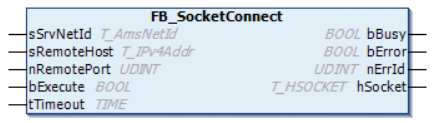
\includegraphics[width=\textwidth]{07_Anlagenmodell/FB_SocketConnect}
				\caption{FB: SocketConnect}
				\label{fig:FB_SocketConnect}
			\end{subfigure}
			\hfill
			\begin{subfigure}[b]{0.45\textwidth}
				\centering
				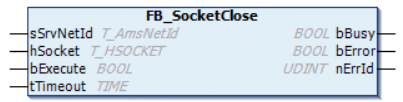
\includegraphics[width=\textwidth]{07_Anlagenmodell/FB_SocketClose}
				\caption{FB: SocketClose}
				\label{fig:FB_SocketClose}
			\end{subfigure}
			\vfill
			\begin{subfigure}[b]{0.45\textwidth}
				\centering
				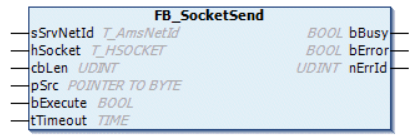
\includegraphics[width=\textwidth]{07_Anlagenmodell/FB_SocketSend}
				\caption{FB: SocketSend}
				\label{fig:FB_SocketSend}
			\end{subfigure}
			\hfill
			\begin{subfigure}[b]{0.45\textwidth}
				\centering
				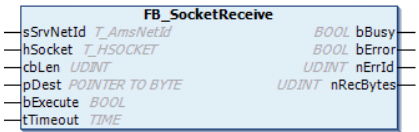
\includegraphics[width=\textwidth]{07_Anlagenmodell/FB_SocketReceive}
				\caption{FB: SocketReceive}
				\label{fig:FB_SocketReceive}
			\end{subfigure}
			\caption{TwinCAT-Funktionsbausteine für TCP/IP}
			\label{fig:TwinCAT-Funktionsbausteine}
		\end{figure}
		
		Für eine detaillierte Beschreibung des TF6310-Pakets kann entsprechende Dokumentation angeschaut werden. 
		\verb|FB_SocketConnect| ist für die Verbindung mit dem Server zuständig. Folgende zwei Informationen werden für die Verbindung zum UR5 benötigt: 
		
		\begin{tabularx}{\textwidth}{@{}>{}p{10em} @{}>{}p{8em} X@{}}
			\verb|sRemoteHoste:| 	& \verb|192.168.1.100|	& IP-Adresse des Roboters 
			\\
			\verb|sRemotePort:| 	& \verb|30002| 			& Verbindung mit Secundary-Schnittstelle
			\\
									& \verb|30003|			& Verbindung mir Real-Time-Schnittstelle
			\\
		\end{tabularx}
		
		Die Variable «\verb|sSrvNetId|» kann mit einem Leerstring versehen werden, da der TwinCAT TCP/IP Connection Server auf dem lokalen Rechner läuft. Sobald der Funktionsbaustein über «\verb|bExecute|» gestartet wird und eine Verbindung zum TCP/IP-Server erfolgreich aufgebaut werden konnte, wird ein TCP/IP-Verbindungshandle erstellt. Dieser wird über «\verb|hSocket|» zur Verfügung gestellt. Über dieses Handle können Daten an einen Socket gesendet oder empfangen werden. Mit \verb|FB_SocketClose| kann die Verbindung zum Kommunikationssocket geschlossen werden.
		\\
		Zum Senden und Empfangen von Daten werden \verb|FB_SocketSend| und \verb|FB_SockerReceive| verwendet. Bede Funktionsbausteine benötigen den definierten TCP/IP-Verbindungshandle, die Anzahl der zu sendenden Daten in Bytes («\verb|cbLen|») und die Pointer-Adresse des Sendepuffers («\verb|pSrc|» / «\verb|pDest|»). 
		\\
		\\
		Die UR5-Objektklasse hat grundsätzlich folgenden Aufgaben: 
		\begin{itemize}
			\item Aufbau und Verwaltung der Verbindung zum UR5-Roboter über TCP/IP
			\item Entgegennahme und Vorbereitung der Prozessdaten
			\item Senden des entsprechenden Befehls an den Roboter, damit eine Bewegung durchgeführt wird
			\item Senden des entsprechenden Befehls an den Roboter, dass eine Bewegung gestoppt werden kann
			\item Entgegennahme, Verarbeitung und Auswertung der vom Roboter gesendeten Daten
		\end{itemize}
		
		\newpage
		
		Für den Aufbau und die Verwaltung der Kommunikation, werden alle relevanten Funktionsbausteine im Bereich «Instanziierungen» der Objektklasse aufgerufen und mit den allgemeinen Variablen verknüpft (\ref{fig:FB_Roboter_SendStart}). Die Zuweisung der Sende- oder Empfangsvariable wird erst innerhalb der entsprechenden Methode vorgenommen. 
		
		\begin{figure}[h!]
			\centering
			\fbox{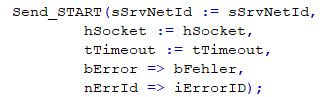
\includegraphics[width=0.5\textwidth]{07_Anlagenmodell/FB_Roboter_SendStart}}
			\captionsetup{justification=centering}
			\caption{Aufrufen eines Funktionsbausteines}
			\label{fig:FB_Roboter_SendStart}
		\end{figure}
		
		Über die Methoden «\verb|M_Verbinden|» und «\verb|M_Trennen|» werden die entsprechenden Trigger der Funktionsbausteine aktiviert um diese auszulösen.  
		Die Prozessdaten, welche durch den Skill zur Verfügung gestellt werden, werden über die Eigenschaft «\verb|P_Prozessparameter|» an das Objekt übergeben. Die Daten werden mittels einer benutzerdefinierten Struktur mit folgender Definition übergeben:
		
		\begin{figure}[h!]
			\centering
			\fbox{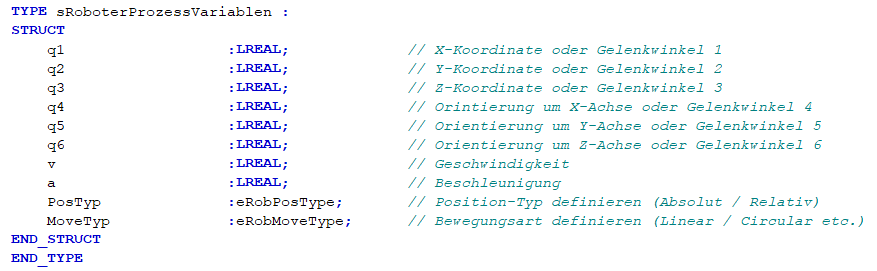
\includegraphics[width=1\textwidth]{07_Anlagenmodell/sRoboterProzessVariablen}}
			\captionsetup{justification=centering}
			\caption{Struktur: sRoboterProzessVariablen}
			\label{fig:sRoboterProzessVariablen}
		\end{figure}
		
		Die Prozessdaten werden innerhalb der Methode «\verb|M_BewegungZuPosition|» analysiert, in die korrekte Form gebracht und versendet.  Die Methode prüft in einem ersten Schritt, um welche Positionsart es sich handelt. Es kann zwischen absolut und relativ unterschieden werden. Je nach Positionsart werden die Koordinaten anders ausgelegt. Der nächste Schritt ist die Bestimmung der Bewegung. Jede Bewegungsart hat einen definierten Befehl in der URScript-Porgrammiersprache. Am Ende kann der Befehl-String zusammengesetzt werden. Ein Befehl-String besteht in der Regel aus dem entsprechenden Befehls-Wort, der Position, der Geschwindigkeit und Beschleunigung. 
		\\
		\\
		Beispiel für einen solchen Befehl-String: 
		
		\begin{tabularx}{\textwidth}{@{}>{}p{12em} @{}>{}p{10em} X@{}}
			\scriptsize 
			\verb|movel(p[x,y,z,rx,ry,rz],a,v)| 	& \verb|movel:|	& Lineare Bewegung im kartesischen Koordinatensystem 
			\\
										& \verb|P[x,y,z,rx,ry,rz]:| & Informationen über anzufahrenden Punkt \verb|[m & rad]|
			\\
													& \verb|a|		& Beschleunigung \verb|[m/s^2]|
			\\
													& \verb|v|		& Geschwindigkeit \verb|[m/s]|
			\\
		\end{tabularx}
		
		\begin{bfhNoteBox}
			Jeder URSript-Befehl muss mit «\verb|\n|» beendet werden. Der String kann aber nicht einfach mit diesen Angaben ergänzt werden. Bei der Umwandlung von einem String in einen Byte-Array wird diese Endung «falsch» übersetzt (mit dem Wert 42). Für die korrekte Interpretation des Befehls durch den Kontroller muss am Ende aber eine 10 stehen. Diese muss dem Byte-Array angehängt werden. Wahrscheinlich ist dies auf unterschiedliche Interpretation von Low- und High-Byte zurückzuführen (die Reihenfolge der Bytes wird dabei vertauscht und führt zu falschen Resultaten). Dies hat zu diversen Problemen geführt in Zusammenhang mit der TCP/IP-Schnittstelle.
		\end{bfhNoteBox}
		
		In folgendem Code-Snippet (\ref{fig:ArrayErgänzung}) wird das Byte-Array mit dem Wert 10 ergänzt und anschliessend über den TCP/IP-Funktionsbaustein «\verb|FB_SocketSend|» an den Server verwendet. 
		
		\begin{figure}[h!]
			\centering
			\fbox{\includegraphics[width=0.7\textwidth]{07_Anlagenmodell/ArrayErgänzung}}
			\captionsetup{justification=centering}
			\caption{Ergänzung von Array}
			\label{fig:ArrayErgänzung}
		\end{figure}
		
		In der Methode \verb|M_BewegungStoppen| wird grundsätzlich dasselbe gemacht. Nur der Befehl-String ändert sich auf den entsprechenden Befehl.
		\\
		Im Bereich «Datenerfassung» wird kontinuierlich der aktuelle Wert der Gelenkposition und Geschwindigkeit erfasst, wie auch die TCP-Position. Die Erfassung arbeitet dabei fortlaufend vier Schritte ab:
		
		\begin{tabularx}{\textwidth}{@{}>{}p{8em} X@{}}
			Schritt 1 & 
			Verbindungsaufbau zu Real-Time-Schnittstelle des Roboters
			\\
			Schritt 2 & 
			Empfangen des Datenpakets (812 Bytes)
			\\
			Schritt 3 & 
			Verarbeitung der Rohdaten   
			\\
			Schritt 4 & 
			Trennung der Verbindung zur Real-Time-Schnittstelle
			\\
		\end{tabularx}
		\\
		
		Erfahrungen haben gezeigt, dass die Schnittstelle immer wieder geschlossen und neu geöffnet werden muss, damit Daten verlässlich ausgelesen werden konnten. Wird dies nicht gemacht, so werden die Daten nur das erste Mal empfangen und behalten anschliessend diese Werte.
		\\
		Ein Positions- oder Geschwindigkeitswert setzen sich jeweils aus 8 Bytes zusammen. Diese können über eine UNION-Datenstruktur zu einem LREAL-Wert zusammengefügt werden. Da TwinCAT die Low- und High-Bytes anders interpretiert als der Roboter-Kontroller, muss die Reihenfolge des Arrays in einem ersten Schritt umgedreht werden. Anschliessend können diese mittels einer UNION-Datenstruktur umgewandelt werden. 
		\\
		Diese Werte werden im Zustand «\verb|LAUFEND|» verwendet, um zu prüfen, ob der Roboter die gewünschte Position bereits erreicht hat. Falls die Differenz zwischen der aktuellen und gewünschten Position einen definierten Grenzwert unterschreitet, gilt die Position als erreicht (\ref{fig:Positionsvergleich}).
		
		\newpage
		
		\begin{figure}[h!]
			\centering
			\fbox{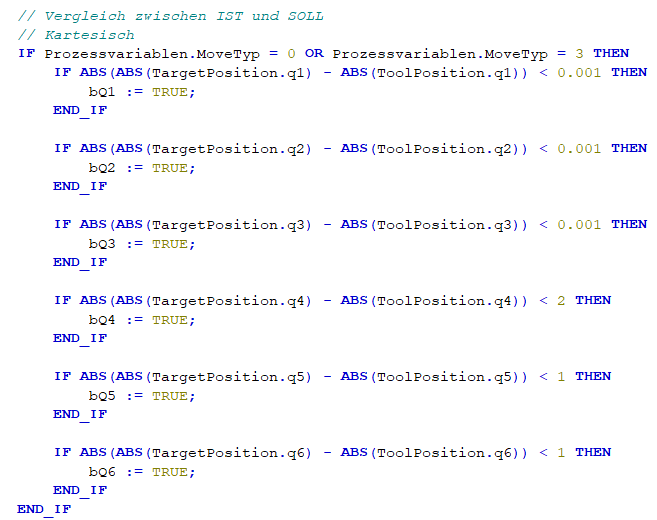
\includegraphics[width=0.7\textwidth]{07_Anlagenmodell/Positionsvergleich}}
			\captionsetup{justification=centering}
			\caption{Vergleich von IST- und SOLL-Positionen}
			\label{fig:Positionsvergleich}
		\end{figure}
		
		Beim Stoppen der Bewegung kann über die aktuelle Geschwindigkeit ermittelt werden, ob der Roboter angehalten hat und somit die Bewegung abgeschlossen wurde.
		\vspace{3mm}
		
		\textbf{Objektklasse für Kraftsensor:} \verb|FB_Kraftsensor|
		\vspace{2mm}
		\vspace{-10mm}  
		\\
		\begin{wrapfigure}{r}{0.5\textwidth}
			\centering
			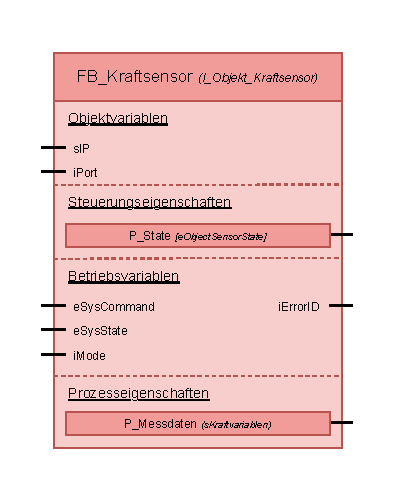
\includegraphics[width=0.45\textwidth]{07_Anlagenmodell/FB_Kraftsensor}
			\captionsetup{justification=centering}
			\caption{Umsetzungsstruktur von Kraftsensor-Objekt}
			\label{fig:Umsetzungsstruktur_Kraftsensorobjekt}
		\end{wrapfigure} \par
		Die Objektklasse (\ref{fig:Umsetzungsstruktur_Kraftsensorobjekt}) implementiert das Interface «\verb|I_Objekt_Kraftsensor|» und gehört zur Kategorie der Sensor-Objekte. Daher enthält sie keine Steuerungsmethoden, sondern lediglich eine Steuerungseigenschaft. Für den Betrieb der Objektklasse sind eine IP-Adresse und eine Port-Nummer als Eingabevariablen erforderlich. Analog zur Roboterobjektklasse werden keine Ausgangsvariablen definiert. Die Kommunikation mit dem Sensor erfolgt ebenfalls über TwinCAT-Funktions-bausteine.
		\\
		Die Steuerungs- und Betriebsvariablen bleiben unverändert gegenüber dem Basis-Funktions-baustein.Die Objektklasse benötigt keine Prozessmethoden. Die Prozesseigenschaft stellt die Messwerte des Sensors zur Verfügung. 
		\\
		\\
		\\
		Wie bereits in Kapitel \ref{Anlagenkomponenten} angesprochen, besitzt der definierte Kraftsensor eine TCP/IP-Schnittstelle. Die Schnittstelle kann verwendet werden, um direkt die Sensor-Rohdaten auszulesen. Um sich mit dem Sensor zu verbinden, muss als Port-Nummer 49151 verwendet werden. 
		\\
		Der Sensor kann Anfragebefehle (20 Bytes) entgegennehmen und Datenpakete (16 Bytes) senden. Dabei ist der Aufbau des Befehls und des Datenpaketes genau vorgegeben. Damit die Daten des Sensors ausgelesen werden können, muss in einem ersten Schritt ein Startbefehl (\ref{tab:Startbefehl_Kraftsensor}) gesendet werden. 
		
		\newcolumntype{L}[1]{>{\raggedright\let\newline\\\arraybackslash\hspace{0pt}}m{#1}}
		\begin{table}[ht]
			\scriptsize
			\centering
			\colorlet{BFH-table}{BFH-MediumBlue!10}
			\colorlet{BFH-tablehead}{BFH-MediumBlue!50}
			\begin{bfhTabular}{| l | c | c | c | L{7.5cm} |}
				Bezeichnung: 		& Sensor-Dt:	& TwinCAT-Dt:		& Byte:			& Wert:
				\\\hline
				\verb|Command|		& UINT8			& UINT				& 1				& Der Wert muss 0 sein
				\\\hline
				\verb|Reserved|		& UINT8			& UNIT				& 19 			& Alle 19 Werte müssen 0 sein 
			\end{bfhTabular}
			\begin{tablenotes}
				\small
				\item (Dt = Datentyp)
			\end{tablenotes}
			\caption{Startbefehl für Kraftsensor}
			\label{tab:Startbefehl_Kraftsensor}
		\end{table}
		
		Der Sensor stellt anschliessend das Datenpaket mit folgender Struktur zur Verfügung: 
		
		\newcolumntype{L}[1]{>{\raggedright\let\newline\\\arraybackslash\hspace{0pt}}m{#1}}
		\begin{table}[ht]
			\scriptsize
			\centering
			\colorlet{BFH-table}{BFH-MediumBlue!10}
			\colorlet{BFH-tablehead}{BFH-MediumBlue!50}
			\begin{bfhTabular}{| l | c | c | c | L{7.5cm} |}
				Bezeichnung: 		& Sensor-Dt:	& TwinCAT-Dt:		& Byte:			& Beschreibung:
				\\\hline
				\verb|Header|		& UINT16		& UINT				& 2				& Ein fixer Wert «0x1234»
				\\\hline
				\verb|Stats|		& UINT16		& UINT				& 2 			& Statuswort des Sensors
				\\\hline
				\verb|Fx|			& INT16			& INT				& 2 			& Kraftwert in X-Richtung  
				\\\hline
				\verb|Fy|			& INT16			& INT				& 2 			& Kraftwert in Y-Richtung  
				\\\hline
				\verb|Fz|			& INT16			& INT				& 2 			& Kraftwert in Z-Richtung  
				\\\hline
				\verb|Tx|			& INT16			& INT				& 2 			& Momentwert um X-Achse
				\\\hline
				\verb|Ty|			& INT16			& INT				& 2 			& Momentwert um Y-Achse
				\\\hline
				\verb|Tz|			& INT16			& INT				& 2 			& Momentwert um Z-Achse 
			\end{bfhTabular}
			\begin{tablenotes}
				\small
				\item (Dt = Datentyp)
			\end{tablenotes}
			\caption{Datenpaket von Sensor}
			\label{tab:Datenpaket_Sensor}
		\end{table}
		
		Die Rohmessdaten müssen nun in Newton und Newton/Meter umgewandelt werden. Dies kann mit folgenden Formeln gemacht werden: 
		
		\newcolumntype{C}[1]{>{\raggedright\let\newline\\\arraybackslash\hspace{0pt}}m{#1}}
		\begin{table}[ht]
			\centering
			\colorlet{BFH-table}{BFH-MediumBlue!10}
			\colorlet{BFH-tablehead}{BFH-MediumBlue!50}
			\begin{bfhTabular}{| C{7cm} | C{7cm} |}
				Umrechnung der Kraft in N: 						& Umrechnung des Moments in N/m:
				\\\hline
				\verb|F(in N) = F * ScaleFactor / CPF|			& \verb|T(in N/m) = T * ScaleFactor / CPT|	
			\end{bfhTabular}
			\captionsetup{justification=centering}
			\caption{Umrechnungsformeln}
			\label{tab:Umrechnungsformeln}
		\end{table}
		
		Alle Faktoren werden durch den Sensor zur Verfügung gestellt, müssen jedoch über eine Anfrage beantragt werden. Mit folgendem Befehl werden die Faktoren gesendet:
		
		\newcolumntype{L}[1]{>{\raggedright\let\newline\\\arraybackslash\hspace{0pt}}m{#1}}
		\begin{table}[!htp]
			\scriptsize
			\centering
			\colorlet{BFH-table}{BFH-MediumBlue!10}
			\colorlet{BFH-tablehead}{BFH-MediumBlue!50}
			\begin{bfhTabular}{| l | c | c | c | L{7.5cm} |}
				Bezeichnung: 		& Sensor-Dt:	& TwinCAT-Dt:		& Byte:			& Wert:
				\\\hline
				\verb|Command|		& UINT8			& UINT				& 1				& Der Wert muss 1 sein
				\\\hline
				\verb|Reserved|		& UINT8			& UNIT				& 19 			& Alle 19 Werte müssen 0 sein 
			\end{bfhTabular}
			\begin{tablenotes}
				\small
				\item (Dt = Datentyp)
			\end{tablenotes}
			\caption{Befehl für Umrechnungsfaktoren}
			\label{tab:Befehl_Umrechnungsfaktoren}
		\end{table}
		
		\newpage
		
		Der Sensor schickt darauf folgend ein Datenpaket mit 24 Byte mit folgender Struktur: 
		
		\newcolumntype{L}[1]{>{\raggedright\let\newline\\\arraybackslash\hspace{0pt}}m{#1}}
		\begin{table}[ht]
			\scriptsize
			\centering
			\colorlet{BFH-table}{BFH-MediumBlue!10}
			\colorlet{BFH-tablehead}{BFH-MediumBlue!50}
			\begin{bfhTabular}{| l | c | c | c | L{7.5cm} |}
				Bezeichnung: 		& Sensor-Dt:	& TwinCAT-Dt:	& Byte:	& Beschreibung:
				\\\hline
				\verb|Header|		& UINT16		& UINT			& 2		& Ein fixer Wert «0x1234»
				\\\hline
				\verb|Unit_Force|	& UINT8			& USINT			& 1 	& Gibt an, welche Einheit mit Faktoren ermittelt wird
				\\\hline
				\verb|Unit_Torque|	& UINT8			& USINT			& 1 	& Gibt an, welche Einheit mit Faktoren ermittelt wird
				\\\hline
				\verb|CPF|			& INT32			& UDINT			& 4 	& Zählwerte pro Kraftwert (Counts per Force value)  
				\\\hline
				\verb|CPT|			& INT32			& UDINT			& 4 	& Zählwerte pro Momentwert (Counts per Torque value) 
				\\\hline
				\verb|ScaleFactorFx|& INT16			& UINT			& 2 	& Skalier-Faktor für Kraft in X-Richtung 
				\\\hline
				\verb|ScaleFactorFy|& INT16			& UINT			& 2 	& Skalier-Faktor für Kraft in Y-Richtung 
				\\\hline
				\verb|ScaleFactorFz|& INT16			& UINT			& 2 	& Skalier-Faktor für Kraft in Z-Richtung 
				\\\hline
				\verb|ScaleFactorTx|& INT16			& UINT			& 2 	& Skalier-Faktor für Moment um X-Achse
				\\\hline
				\verb|ScaleFactorTy|& INT16			& UINT			& 2 	& Skalier-Faktor für Moment um Y-Achse
				\\\hline
				\verb|ScaleFactorTz|& INT16			& UINT			& 2 	& Skalier-Faktor für Moment um Z-Achse 
			\end{bfhTabular}
			\begin{tablenotes}
				\small
				\item (Dt = Datentyp)
			\end{tablenotes}
			\caption{Datenpaket von Sensor für Umrechnungsfaktoren}
			\label{tab:Datenpaket_Sensor_Umrechnungsfaktoren}
		\end{table}
		
		Folgende Faktoren werden für die Umrechnung in Newton und Newton/Meter verwendet: 
		
		\begin{tabularx}{\textwidth}{@{}>{}p{8em} @{}>{}p{8em} @{}>{}p{10em}}
			& CPF = 10000 		& ScaleFactorFx = 200
			\\
			& CPT = 10000 		& ScaleFactorFy = 200
			\\
			& 					& ScaleFactorFz = 200
			\\
			& 					& ScaleFactorTx = 100
			\\
			& 					& ScaleFactorTy = 100
			\\
			& 					& ScaleFactorTz = 65
			\\
		\end{tabularx}
		
		In TwinCAT wird wieder mit dem Paket TF6310 (TwinCAT 3 | TCP/IP) gearbeitet, um die Kommunikation zum Sensor aufzubauen. Der Sensor stellt hierbei wieder den Server dar. Entsprechend können die gleichen vier Funktionsbausteine wie beim Roboter verwendet werden.
		\\
		Für die Verbindung zum Server mittels \verb|FB_SocketConnect| werden folgende zwei Informationen benötigt: 
		
		\begin{tabularx}{\textwidth}{@{}>{}p{10em} @{}>{}p{8em} X@{}}
			\verb|sRemoteHoste:| 	& \verb|192.168.1.10|	& IP-Adresse des Sensors 
			\\
			\verb|sRemotePort:| 	& \verb|49151| 			& Port für TCP-Schnittstelle 
			\\
		\end{tabularx}
		\\
		
		Die allgemeine Verwendung der Kommunikationsbausteine bleibt identisch zum Roboter, wie auch der Aufbau der Objektklasse. Die Kraftsensor-Objektklasse hat grundsätzlich folgenden Aufgaben: 
		\begin{itemize}
			\item Aufbau und Verwaltung der Verbindung zum Sensor über TCP/IP
			\item Entgegennahme, Verarbeitung und Auswertung der vom Sensor gesendeten Daten
		\end{itemize}
		
		Die Objektklasse wertet grundsätzlich die Sensordaten aus, wandelt die Rohdaten um und stellt diese über die Prozesseigenschaft zur Verfügung. Der Prozess der Datenauslesung ist dabei wieder in 4 Schritte aufgeteilt: 
		
		\begin{tabularx}{\textwidth}{@{}>{}p{8em} X@{}}
			Schritt 1 & 
			Verbindungsaufbau zu Sensor über TCP/IP
			\\
			Schritt 2 & 
			Empfangen des Datenpakets (16 Bytes)
			\\
			Schritt 3 & 
			Verarbeitung der Rohdaten   
			\\
			Schritt 4 & 
			Trennung der Verbindung von TCP/IP-Schnittstelle
			\\
		\end{tabularx}
		\\
		\newpage
		
		Auch hier musste berücksichtigt werden, dass die Low- und High-Bytes von TwinCAT anders interpretiert, als vom Server vorgesehen. Da der Messwert nur aus zwei Byte besteht, kann dies relativ simpel gemacht werden. Das Prinzip ist wie folgt:
		
		\begin{figure}[h!]
			\centering
			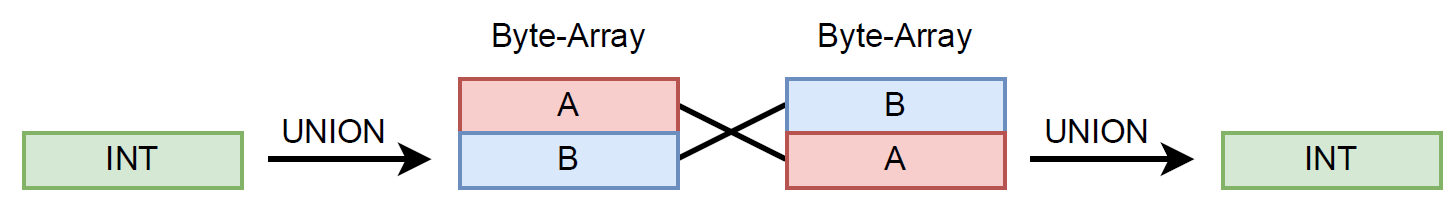
\includegraphics[width=1\textwidth]{07_Anlagenmodell/ByteSwitch}
			\caption{Byte-Switch von Low- und High-Byte}
			\label{fig:ByteSwitch}
		\end{figure} 
		
		Der über die Kommunikationsschnittstelle erhaltene INT-Wert wird mittels eines UNION-Datentyps in eine Array mit zwei Byte umgewandelt. Die Reihenfolge der Bytes wird umgedreht, damit das Array anschliessend mit einem weiteren UNION-Datentyp, in eine INT-Variable zurückgewandelt wird. Der nun korrekte Rohwert kann jetzt für die Umwandlung in den entsprechende Einheit verwendet werden.  In TwinCAT sieht dies folgendermassen aus: 
		
		\begin{figure}[h!]
			\centering
			\fbox{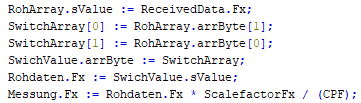
\includegraphics[width=0.6\textwidth]{07_Anlagenmodell/ByteSwitchCode}}
			\captionsetup{justification=centering}
			\caption{Code für Byte-Switch}
			\label{fig:ByteSwitchCode}
		\end{figure} 
		
		Die umgewandelten Daten werden über die Prozesseigenschaft «\verb|P_Messdaten|» zur Verfügung gestellt werden. Für den Datentyp der Eigenschaft wurde die Struktur «\verb|sKraftvariablen|» angegeben. Diese benutzerdefinierte Struktur ist wie folgt definiert: 
		
		\begin{figure}[h!]
			\centering
			\fbox{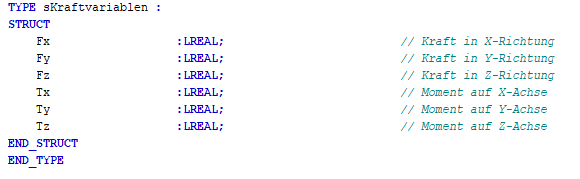
\includegraphics[width=0.8\textwidth]{07_Anlagenmodell/sKraftvariablen}}
			\captionsetup{justification=centering}
			\caption{Struktur: sKraftvariablen}
			\label{fig:sKraftvariablen}
		\end{figure} 
		
		\newpage
		
		\textbf{Objektklasse für Greifer (mit Sensoren):} \verb|FB_SmartGreifer|
		\vspace{2mm}
		\vspace{-10mm}  
		\\
		\begin{wrapfigure}{r}{0.5\textwidth}
			\centering
			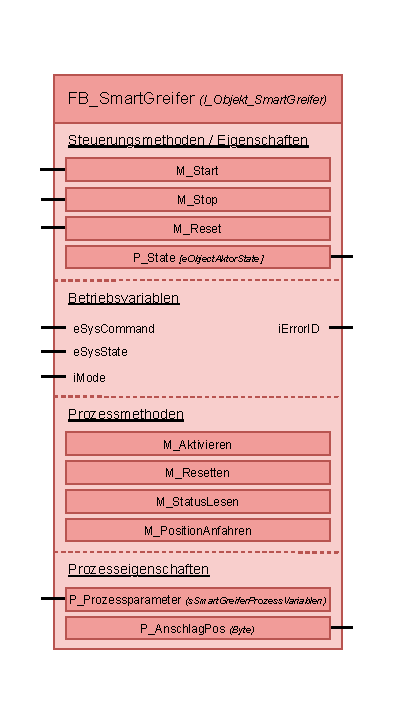
\includegraphics[width=0.45\textwidth]{07_Anlagenmodell/FB_SmartGreifer}
			\captionsetup{justification=centering}
			\caption{Umsetzungsstruktur von Greifer-Objekt}
			\label{fig:Umsetzungsstruktur_SmartSensorobjekt}
		\end{wrapfigure} \par
		Die letzte Objektklasse (\ref{fig:Umsetzungsstruktur_SmartSensorobjekt}) wird mit dem Interface «\verb|I_Objekt SmartGreifer|» implementiert. Da es sich beim Objekt wieder um einen Aktor handelt, werden durch das Interface auch Steuerungsmethoden vorgegeben. Die Objektklasse besitzt keine Objektvariablen. Die Kommunikation zum Greifer wird über TwinCAT-Funktions-bausteine aufgebaut, welche direkt auf EA-Klemmen zugreifen. 
		\\
		Die Steuerungs- und Betriebsvariablen bleiben unverändert zum Basis-Funktionsbaustein.
		\\
		Als Prozessmethoden für den Funktionsbaustein wurden \verb|M_Aktivieren|, \verb|M_Resetten|, \verb|M_StatusLesen|
		und \verb|M_Position_Anfahren| definiert. Diese Funktionen decken die Grundfunktionalitäten des Greifers ab. Durch die Methoden kann eine bestimmte Backenposition angefahren werden und überprüft werden, ob diese Position erreicht wurde, oder wann der Greifer in ein Hindernis gefahren ist.
		\\
		Mit den Prozesseigenschaften werden die prozessrelevanten Parameter für den Greifer definiert. Über \verb|P_AnschlagPos|  wird die Backenposition zur Verfügung gestellt, bei welcher der Greifer in eine Hindernis gefahren ist. 
		\\
		Die Kommunikation zum Greifer wird über ein Modbus RTU Protokoll realisiert. Innerhalb der Dokumentation wird nicht weiter auf die Spezifikation dieses Protokolls eingegangen. Bei der Kommunikation handelt es sich um eine Master-Slave-Kommunikation. Der Greifer stellt dabei den Slave dar. Die wichtigsten Eigenschaften, welche die Verbindung zum Greifer einhalten muss, sind folgende:
		
		\begin{tabularx}{\textwidth}{@{}>{}p{13em} X@{}}
			Anschlussschnittstelle: & 
			RS-485
			\\
			Baud-Rate: & 
			115200 bps (Bits per Second)
			\\
			Data-Bits: & 
			8 Bits 
			\\
			Stop-Bits: & 
			1 Bit 
			\\
			Parität: & 
			Keine
			\\
			Slave-ID: & 
			9
			\\
			Packetgrösse: & 
			2 Byte (16 bit)
			\\
		\end{tabularx} \vspace{3mm} 
		
		Die Modbus RTU Schnittstelle des Greifers unterstützt verschiedene Funktionalitäten, welche unterschiedliche Register darstellen, auf welche man zugreifen kann. Die Register haben unterschiedliche Anfragebefehle und Antworten. Um die Kommunikationsschnittstelle korrekt anwenden zu können, ist es wichtig diese Funktionalitäten und Ihre Befehle und Antworten zu verstehen. Der genaue Aufbau der Nachricht und Antwort kann aus der Dokumentation des Greifers entnommen werden.
		
		\newpage
		
		Als Beispiel wird der Befehl für das komplette Schliessen des Greifers bei 100\verb|%| Geschwindigkeit und Kraft gezeigt:  
		\newcolumntype{L}[1]{>{\raggedright\let\newline\\\arraybackslash\hspace{0pt}}m{#1}}
		\begin{table}[ht]
			\scriptsize
			\centering
			\colorlet{BFH-table}{BFH-MediumBlue!10}
			\colorlet{BFH-tablehead}{BFH-MediumBlue!50}
			\begin{bfhTabular}{| c | c | L{11.5cm} |}
				Array-Nr. 	& Bits (Hex):& Beschreibung:		
				\\\hline
				0			& 09		& Slave-ID				
				\\\hline
				1			& 10		& Funktionscode 16 (Preset Multiple Registers)			
				\\\hline
				2 + 3		& 03 E8		& Adresse des ersten Registers			 
				\\\hline
				4 + 5		& 00 03		& Anzahl der zu beschreibenden Register
				\\\hline
				6			& 06		& Anzahl der Daten-Bytes (3 Register x 2 Bytes = 6 Bytes)			
				\\\hline
				7 + 8		& 09 00		& Wert auf Register schreiben (Aktivieren von Greifer)
				\\\hline
				9 + 10	 	& 00 FF		& Wert auf Register schreiben (Position für komplett geschlossenen Greifer angeben 255/255)
				\\\hline
				11 + 12	 	& FF FF		& Wert auf Register Schreiben (100\verb|%| Geschwindigkeit und Kraft)
				\\\hline
				13 + 14		& 42 29		& Zyklische Redundanzprüfung (CRC)		
			\end{bfhTabular}
			\caption{Beispiel für das Schliessen des Greifers}
			\label{tab:Greifer_Beispiel}
		\end{table}
		
		Die Interaktion mit dem Greifer über die herstellereigene Software funktionierte einwandfrei. Der Greifer wurde über einen RS-485-USB-Adapter am PC angeschlossen. Der Greifer-Port wurde sofort erkannt und konnte verwendet werden. Auch über Programme wie „Modbustester“ konnte der Greifer verbunden und getestet werden. Die Integration des Greifers in TwinCAT via Modbus RTU war jedoch eine aufwändige und zeitintensive Arbeit. TwinCAT stellt grundsätzlich ein Paket für die Kommunikation mit Modbus RTU zur Verfügung, TF6255 (TwinCAT 3 | Modbus RTU). Das Paket stellt verschiedene Funktionsbausteine für die Kommunikation zur Verfügung. Einer dieser Funktionsbausteine stellt die Verbindung über eine COM-Port-Schnittstelle auf. Nach endlosen versuchen war es aber nicht möglich eine Verbindung mit dem Greifer aufzubauen. Mit Hilfe einer Software zur Überwachung von Serial-Port-Schnittstellen wurde festgestellt, dass kein Signal TwinCAT verlässt. Es wurde kein Weg gefunden eine Verbindung über eine COM-Port-Schnittstelle mittels TwinCAT zum Greifer herzustellen.
		\\
		\vspace{-5mm} 
		\begin{wrapfigure}{r}{0.55\textwidth}
			\centering
			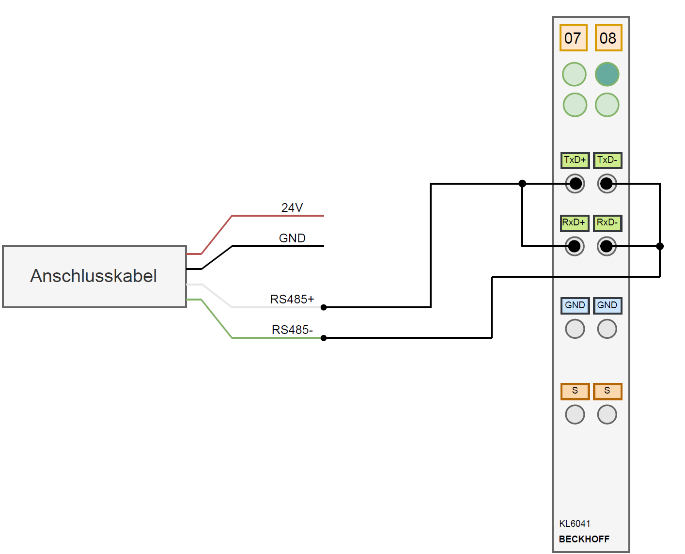
\includegraphics[width=0.45\textwidth]{07_Anlagenmodell/Kartenanschluss}
			\captionsetup{justification=centering}
			\caption{Anschluss der Beckhoff-Karte}
			\label{fig:KL6041}
		\end{wrapfigure}
		Als Alternative wurde versucht sich über eine RS-485-Interface-Karte von Beckhoff mit dem Greifer zu verbinden. Dafür wurde die KL6041 (1-Kanal-Kommunikations-interface) ausgewählt. Wichtig beim Anschluss der Karte ist, dass der Greifer als «Half-Duplex» angeschlossen werden muss (\ref{fig:KL6041}). Dabei wird die Datenleitung für das Sensen und Empfangen verwendet. Im aufgeführten Schema wird dargestellt, wie die Klemme mit den entsprechenden Anschlüssen des Kabels verbunden werden müssen. Über einen Busskoppler (BK1120) kann die Karte über eine EtherCAT-Schnittstelle ausgewertet werden. Es war schlussendlich möglich, den Greifer über die KL6041-Karte anzusteuern und Daten auszulesen. 
		
		\newpage
		
		Die Karte muss mit dem Konfigurationstool KS2000 von Beckhoff (\ref{fig:KS2000}) korrekt konfiguriert werden. Anschliessend  kann diese verknüpft und eingesetzt werden. 
		
		\begin{figure}[H]
			\centering
			
\includegraphics[width=.8\textwidth]{placeholder}
			\captionsetup{justification=centering}
			\caption{KS2000-Konfigurationstool}
			\label{fig:KS2000}
		\end{figure}
		
		Das Paket TF6255 stellt für den Einsatz einer KL6041-Karte einen separaten Funktionsbaustein zur Verfügung (\ref{fig:FB_ModbusRTU}).
		
		\begin{figure}[H]
			\centering
			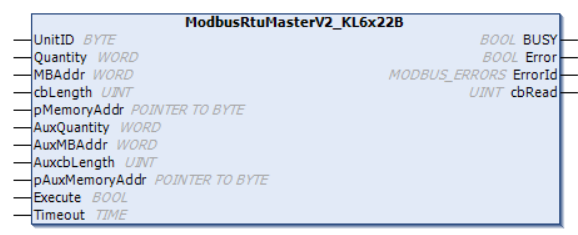
\includegraphics[width=.7\textwidth]{07_Anlagenmodell/FB_ModbusRTU}
			\captionsetup{justification=centering}
			\caption{Kommunikationsbaustein für Modbus RTU}
			\label{fig:FB_ModbusRTU}
		\end{figure}
		
		Der Funktionsbaustein erstellt anhand der Eingangsvariablen den zu sendenden Befehlsframe für die Modbus RTU Kommunikation. Folgende Eingangsvariabel sind relevant für die korrekte Erstellung des Frames:
		
		\newcolumntype{L}[1]{>{\raggedright\let\newline\\\arraybackslash\hspace{0pt}}m{#1}}
		\begin{table}[ht]
			\scriptsize
			\centering
			\colorlet{BFH-table}{BFH-MediumBlue!10}
			\colorlet{BFH-tablehead}{BFH-MediumBlue!50}
			\begin{bfhTabular}{| l | l | L{5cm} |}
				Bezeichnung	& Beschreibung								& Beispielwert (Tabelle X)		
				\\\hline
				UnitID		& Slave-ID des Greifers 					& 09 (Hex) | 9 (Dez)				
				\\\hline
				Quantity	& Anzahl der zu beschreibenden Register 	& 03 (Hex) | 3 (Dez)
				\\\hline
				MBAddr		& Adresse des ersten Registers				& 03E8 (Hex) | 1000 (Dez) 		 
				\\\hline
				cbLenght	& Anzahl der zu sendenden Daten in Bytes	& 06 (Hex) | 6 (Dez)
			\end{bfhTabular}
			\captionsetup{justification=centering}
			\caption{Eingabeparameter für Funktionsbaustein}
			\label{tab:Eingabeparameter_ModbusRTU}
		\end{table}
		
		\newpage
		
		Der folgende Bildausschnitt aus der Methode \verb|M_PositionAnfahren| veranschaulicht, wie eine entsprechende Implementierung in TwinCAT aussehen kann. Die Slave-ID wurde dabei bereits übergeordnet definiert, da sie für alle Befehle unverändert bleibt.
		
		\begin{bfhNoteBox}
			Ein wichtiger Aspekt bei der Zusammenstellung der Daten für die Register ist die Problematik von High- und Low-Bit. Die Registerdaten sind im Vergleich zur Dokumentation des Greifers vertauscht. Konkret bedeutet dies, dass die Array-Nummern aus dem Beispiel (Tabelle X) [7, 8, 9, 10, 11, 12] in TwinCAT zu [8, 7, 10, 9, 12, 11] angepasst werden müssen. Das gleiche Prinzip gilt auch für das Auslesen der Register.
		\end{bfhNoteBox}
		\vspace{3mm} 
		Der Funktionscode wird durch die ausgewählte Aktion des Funktionsblocks definiert. Für dieses Beispiel (\ref{fig:FB_Anwenung_Kommunikation}) wurde der Funktionscode 16 «Communication.WriteRegs» ausgewählt. Der Basis-Funktionsbaustein, in diesem Fall «Communication» kann nicht in seiner Grundform aufgerufen werden, sondern nur zusammen mit einer Aktion. 
		
		\begin{figure}[H]
			\centering
			\fbox{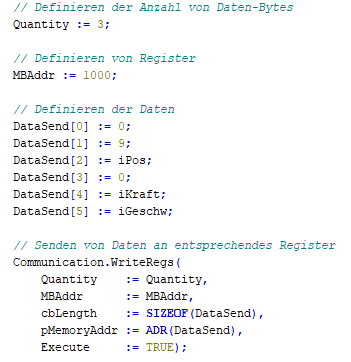
\includegraphics[width=.5\textwidth]{07_Anlagenmodell/WriteRegs}}
			\captionsetup{justification=centering}
			\caption{Anwendung des Kommunikationsbausteines}
			\label{fig:FB_Anwenung_Kommunikation}
		\end{figure}
		
		
		
		